\begin{correction}  \;
\begin{enumerate}
\item La fonction $f$ est d\'efinie sur $\R$.
\begin{itemize}
\item[$\bullet$] \'Etude de la parit\'e: $\R$ est centr\'e en 0. Soit $x\in\R$: $f(-x)=3\cos{(-x)}-\cos{(-3x)}=3\cos{x}-\cos{(3x)}$ car la fonction $f$ est paire. Ainsi $f(-x)=f(x)$, et la fonction $f$ est paire.
\item[$\bullet$] \'Etude de la p\'eriodicit\'e: v\'erifions que la fonction est $2\pi$ p\'eriodique:
\begin{itemize}
\item[$\star$] Pour tout $x\in\R$, $x+2\pi\in\R$. 
\item[$\star$] Soit $x\in\R$: $f(x+2\pi)=3\cos{(x+2\pi)}-\cos{(3(x+2\pi))}=3\cos{(x+2\pi)}-\cos{(3x+6\pi)}=f(x)$ en utilisant la $2\pi$ p\'eriodicit\'e de la fonction cosinus.
\end{itemize}
Ainsi la fonction $f$ est $2\pi$ p\'eriodique. 
\end{itemize}
Par $2\pi$ p\'eriodicit\'e, on peut restreindre l'\'etude \`{a} tout intervalle d'amplitude $2\pi$, par exemple $\lbrack -\pi,\pi\rbrack$. Puis par parit\'e, on peut restreindre l'intervalle \`{a} $\lbrack 0,\pi\rbrack$. La courbe $\mathcal{C}_f$ sera alors obtenue par sym\'etrie par rapport \`{a} l'axe des ordonn\'ees puis par translation de vecteur $2\pi\vec{i}$. 
\item La fonction $f$ est d\'erivable sur $\R$ comme compos\'ee et somme de fonctions d\'erivables. Pour tout $x\in\R$, on a: $f^{\prime}(x)=-3\sin{x}+3\sin{(3x)}=-3( \sin{x}-\sin{(3x)} )= -3 \times 2\cos{(2x)}\sin{( -x)}=6\cos{(2x)}\sin{( x)} $ en utilisant une formule de trigonom\'etrie et le fait que la fonction sinus est impaire. 
\item  \'Etude du signe de $f^{\prime}$ sur $\lbrack 0,\pi\rbrack$:\\
\noindent Sur $\lbrack 0,\pi\rbrack$, on a: $\sin{(x)}\geq 0$ et ainsi le signe de $f^{\prime}$ ne d\'epend que du signe de $\cos{(2x)}$. On a: $\cos{(2x)}\geq 0\Leftrightarrow \exists k\in\Z,\ -\ddp\frac{\pi}{2}+2k\pi\leq 2x \leq \ddp\frac{\pi}{2}+2k\pi\Leftrightarrow \exists k\in\Z,\ -\ddp\frac{\pi}{4}+k\pi\leq x \leq \ddp\frac{\pi}{4}+k\pi$. En faisant un cercle trigonom\'etrique, on remarque que sur $\lbrack 0,\pi\rbrack$, on obtient: $\cos{(2x)}\geq 0\Leftrightarrow x\in\lbrack 0,\ddp\frac{\pi}{4}\rbrack\cup \lbrack \ddp\frac{3\pi}{4},\pi\rbrack$. On obtient ainsi le tableau des variation suivant:
\begin{center}
 \begin{tikzpicture}
 \tkzTabInit{ $x$          /1,%
      $f^{\prime}(x)$   /1,
       $f$       /2}%
     { $0$,$\ddp\frac{\pi}{4}$,$\ddp\frac{3\pi}{4}$,$\pi$}%
   \tkzTabLine{ ,+,0,-,0,+,}
  \tkzTabVar{
       -/$2$            /,
       +/$2\sqrt{2}$         /,
        -/$-2\sqrt{2}$         /,
        +/$-2$         /,
                              }                
\end{tikzpicture}
\end{center}
\item 
\begin{itemize}
\item[$\bullet$] La fonction $f$ est d\'erivable en $\ddp\frac{\pi}{2}$ donc la tangente \`{a} la courbe $\mathcal{C}_f$ au point d'abscisse $\ddp\frac{\pi}{2}$ existe bien et son \'equation est: $y=f^{\prime}(\ddp\frac{\pi}{2}) (x-\ddp\frac{\pi}{2})+f(\ddp\frac{\pi}{2})$. On obtient ainsi: $y=-6(x-\ddp\frac{\pi}{2})$.
\item[$\bullet$] La tangente est horizontale lorsque $f^{\prime}(x)=0$. On obtient donc: $f^{\prime}(x)=0\Leftrightarrow \cos{(2x)}=0\ \hbox{ou}\ \sin{x}=0\Leftrightarrow \exists k\in\Z,\ x=\ddp\frac{\pi}{4}+\ddp\frac{k\pi}{2}\ \hbox{ou}\ \exists k\in\Z,\ x=k\pi$.
\end{itemize}
%\item Graphe de $f$ :
%\begin{center}
%\includegraphics[width=0.5\linewidth]{./ex15.eps} 
%\end{center}
\end{enumerate}
\end{correction}



%----------------------------------------------------------------------------------------------
%-----------------------------------------------------------------------------------------------
%----------------------------------------------------------------------------------------------
%-----------------------------------------------------------------------------------------------
%\section{Avec les fonctions usuelles}
%--------------------------------------------------
%------------------------------------------------
%\begin{correction}
%\begin{itemize}
%\item[$\bullet$] La fonction $f$ est bien d\'efinie si et seulement si $x>0$ et $x(\ln{x}+1)\not= 0$. On a: $x(\ln{x}+1)\not= 0\Leftrightarrow x\not= 0\ \hbox{et}\ \ln{x}\not= -1$. Et on a: $\ln{x}\not= -1\Leftrightarrow x\not= e^{-1}$ car la fonction exponentielle est strictement croissante sur $\R$. Ainsi on obtient que: $\mathcal{D}_f=\rbrack 0,e^{-1}\lbrack\cup\rbrack e^{-1},+\infty\lbrack$.
%\item[$\bullet$] \'Etude des limites aux bornes du domaine de d\'efinition:
%\begin{itemize}
%\item[$\star$] Limite en $0^+$: Au d\'enominateur, on a une FI. Mais on a: $x(\ln{x}+1)=x\ln{x}+x$. Par croissance compar\'ee, on obtient que: $\lim\limits_{x\to 0^+} x\ln{x}=0$. Ainsi par somme de limites, on obtient que: $\lim\limits_{x\to 0^+} x(\ln{x}+1)=0$. Comme on est au d\'enominateur, on a besoin de savoir si c'est $0^+$ ou $0^-$. On fait pour cela un tableau de signe et on obtient:
%\begin{center}
% \begin{tikzpicture}
% \tkzTabInit[lgt=3]{ $x$          /,%
%      $x$   /,
%       $\ln{x}+1$       /,
%       $x(\ln{x}+1)$     /}%
%     { $0$,$e^{-1}$,$+\infty$}%
%   \tkzTabLine{ 0,$+$,t,$+$,}  
%   \tkzTabLine{ d,$-$,0,$+$,} 
%   \tkzTabLine{ d,$-$,0,$+$,}    
%\end{tikzpicture}
%\end{center}
%Ainsi, on a: $\lim\limits_{x\to 0^+} x(\ln{x}+1)=0^-$. Puis par propri\'et\'e sur les somme et quotient de limites, on obtient que: $\lim\limits_{x\to 0^+} f(x)=+\infty$.
%\item[$\star$] Limite en $e^{-1}$: toujours en s'aidant du tableau de signe ci-dessus, on obtient: $\lim\limits_{x\to (e^{-1})^-} x(\ln{x}+1)=0^-$ et $\lim\limits_{x\to (e^{-1})^+} x(\ln{x}+1)=0^+$. Puis comme $e^{-1}-1<0$, on obtient: $\lim\limits_{x\to (e^{-1})^-}  f(x)=+\infty$ et $\lim\limits_{x\to (e^{-1})^+}  f(x)=-\infty$.
%\item[$\star$] Limite en $+\infty$: en mettant en facteur le terme dominant au num\'erateur et au d\'enominateur, on obtient: $f(x)=\ddp\frac{x(1-\frac{1}{x})}{  x\ln{x} (1+\frac{1}{\ln{x}}) }=\ddp\frac{1-\frac{1}{x}}{  \ln{x} (1+\frac{1}{\ln{x}}) }$. Ainsi par propri\'et\'e sur les somme, produit et quotient de limite, on obtient: $\lim\limits_{x\to +\infty} f(x)=0$.
%\end{itemize}
%\item[$\bullet$] \'Etude de la d\'erivabilit\'e: la fonction $f$ est d\'erivable sur $\mathcal{D}_f$ comme somme, produit et quotient dont le d\'enominateur ne s'annule pas de fonctions d\'erivables. De plus, pour tout $x\in\mathcal{D}_f$, on obtient: $f^{\prime}(x)=\ddp\frac{x(\ln{x}+1) -(x-1)(\ln{(x)} +2) }{x^2(  \ln{x}+1 )^2}=\ddp\frac{  \ln{x}-x+2}{x^2(  \ln{x}+1 )^2}$. 
%\item[$\bullet$] \'Etude du signe de $f^{\prime}$: le d\'enominateur est un carr\'e donc il est toujours positif. Le signe de $f^{\prime}$ d\'epend donc uniquement du signe de son num\'erateur \`{a} savoir du signe de $\ln{x}-x+2$. On ne sait pas \'etudier directement le signe d'une telle expression, on va donc \'etudier les variations de cette fonction pour en d\'eduire son signe. On pose pour cela: $g(x)=\ln{x}-x+2$. 
%\begin{itemize}
%\item[$\star$] La fonction $g$ est bien d\'efinie sur $\R^{+\star}$ et elle est bien d\'erivable sur $\R^{+\star}$ comme somme de fonctions d\'erivables. Pour tout $x>0$, on a: $g^{\prime}(x)=\ddp\frac{1}{x}-1=\ddp\frac{1-x}{x}$. 
%\item[$\star$] \'Etude des limites en $0$ et en $+\infty$:\\
%\noindent Par propri\'et\'e sur les somme de limites, on a: $\lim\limits_{x\to 0^+} g(x)=-\infty$.\\
%\noindent On met en facteur le terme dominant, \`{a} savoir $x$ dans l'expression de $g$ afin de lever l'ind\'etermination, on obtient: $g(x)=x\left( \ddp\frac{\ln{x}}{x}-1+\ddp\frac{2}{x} \right)$. Par croissance compar\'ee, on a: $\lim\limits_{x\to +\infty} \ddp\frac{\ln{x}}{x}=0$ puis par propri\'et\'e sur les quotients, sommes et produit de limites, on a: $\lim\limits_{x\to +\infty} g(x)=-\infty$.
%\item[$\star$] On obtient ainsi les variations suivantes pour $g$ en remarquant que $g(1)=1$:
%\begin{center}
% \begin{tikzpicture}
% \tkzTabInit{ $x$          /,%
%      $g^{\prime}(x)$   /,
%       $g$       /2}%
%     { $0$,$1$,$+\infty$}%
%   \tkzTabLine{ ,$+$,0,$-$,}
%  \tkzTabInit{
%       -/ $-\infty$           /,
%       +/$1$         /,
%        -/ $-\infty$    /,
%        }
%%        -/         /,
%%        +/$+\infty$         /,
%%                      }
%%\valeur[draw]{1}{3}{1}{}{}   
%%\tkzTabTan[pos=below]{1}{3}{2}{$0$}   
%%\valeur[draw]{1}{3}{1}{$0$}   
%%\tkzTabTan[pos=below]{1}{3}{2}{$0$}           
%\tkzTabInit[draw]{1}{2}{0.4}{$\alpha$}{$0$}                      
%\tkzTabInit[draw]{2}{3}{0.4}{$\beta$}{$0$}                                
%\end{tikzpicture}
%\end{center}
%\item[$\star$] \'Etude du signe de $g$:
%\begin{itemize}
%\item On a:\\
%\noindent La fonction $g$ est continue sur $\rbrack 0,1\lbrack$ comme somme de fonctions continues.\\
%\noindent La fonction $g$ est strictement croissante sur $\rbrack 0,1\lbrack$.\\
%\noindent $\lim\limits_{x\to 0} g(x)=-\infty$ et $g(1)=1$.\\
%\noindent Ainsi d'apr\`{e}s le th\'eor\`{e}me de la bijection, la fonction $g$ est bijective de $\rbrack 0,1\lbrack$ dans $\rbrack -\infty,1\lbrack$. Comme $0\in \rbrack -\infty,1\lbrack$, il existe bien un unique $\alpha\in \rbrack 0,1\lbrack$ tel que $g(\alpha)=0$.
%\item On a:\\
%\noindent La fonction $g$ est continue sur $\rbrack 1,+\infty\lbrack$ comme somme de fonctions continues.\\
%\noindent La fonction $g$ est strictement d\'ecroissante sur $\rbrack 1,+\infty\lbrack$.\\
%\noindent $\lim\limits_{x\to +\infty} g(x)=-\infty$ et $g(1)=1$.\\
%\noindent Ainsi d'apr\`{e}s le th\'eor\`{e}me de la bijection, la fonction $g$ est bijective de $\rbrack 1,+\infty\lbrack$ dans $\rbrack -\infty,1\lbrack$. Comme $0\in \rbrack -\infty,1\lbrack$, il existe bien un unique $\beta\in \rbrack 1,+\infty \lbrack$ tel que $g(\beta)=0$.
%\end{itemize}
%On en d\'eduit le signe de $g$:
%\begin{center}
% \begin{tikzpicture}
% \tkzTabInit{ $x$          /,%
%     % $g^{\prime}(x)$   /,
%       $g$       /2}%
%     { $0$,$\alpha$,$\beta$,$+\infty$}%
%   \tkzTabLine{ ,$-$,0,$+$,0,$-$,}        
%\end{tikzpicture}
%\end{center}
%Il reste alors \`{a} savoir o\`{u} est $e^{-1}$ par rapport \`{a} $\alpha$: on remarque que $g(e^{-1})=1-e^{-1}>0$. Ainsi le th\'eor\`{e}me de la bijection permet d'obtenir: $\alpha<e^{-1}$.
%\end{itemize}
%\item[$\bullet$] Variations de $f$:
%\begin{center}
% \begin{tikzpicture}
% \tkzTabInit{ $x$          /,%
%      $f^{\prime}(x)$   /,
%       $f$       /2}%
%     { $0$,$\alpha$,$e^{-1}$,$\beta$,$+\infty$}%
%   \tkzTabLine{ ,$-$,0,$+$,d,$+$,0,$-$,}
%  \tkzTabInit{
%       +/$+\infty$            /,
%       -/$f(\alpha)$      /,
%       +D-/$+\infty$/$-\infty$         /,
%       +/$f(\beta)$         /,
%        -/$0$     /,
%        }
%\end{tikzpicture}
%\end{center}
%\item[$\bullet$] Calcul de $f(\alpha)$ et $f(\beta)$: Ces deux nombres sont d\'efinis par: $g(\alpha)=g(\beta)=0$ ainsi on sait que: $\ln{\alpha}-\alpha+2=0\Leftrightarrow \ln{\alpha}=\alpha-2$ et $\ln{\beta}-\beta+2=0\Leftrightarrow \ln{\beta}=\beta-2$. Ainsi, on a: $f(\alpha)=\ddp\frac{\alpha-1}{\alpha( \alpha-2+1 )}=\ddp\frac{\alpha-1}{\alpha( \alpha-1 )}=\ddp\frac{1}{\alpha}$. De m\^{e}me, on a: $f(\beta)=\ddp\frac{1}{\beta}$.
%
%
%\end{itemize}
%\end{correction}
%--------------------------------------------------
%------------------------------------------------
%\begin{correction}
%\begin{itemize}
%\item[$\bullet$] La fonction $f$ est bien d\'efinie si et seulement si $1+\ddp\frac{1}{x}>0\Leftrightarrow \ddp\frac{x+1}{x}>0$. Ainsi $\mathcal{D}_f=\rbrack -\infty, -1\lbrack\cup\rbrack 0,+\infty\lbrack$.
%\item[$\bullet$] \'Etude des limites aux bornes:
%\begin{itemize}
%\item[$\star$] \'Etude en $-\infty$: par propri\'et\'e sur les monomes de plus haut degr\'e, on a: $\lim\limits_{x\to -\infty} \ddp\frac{x+1}{x}=1$ et ainsi par propri\'et\'e sur les compos\'e et somme de limites, on obtient que: $\lim\limits_{x\to -\infty} f(x)=-\infty$.
%\item[$\star$] \'Etude en $+\infty$: par propri\'et\'e sur les monomes de plus haut degr\'e, on a: $\lim\limits_{x\to +\infty} \ddp\frac{x+1}{x}=1$ et ainsi par propri\'et\'e sur les compos\'e et somme de limites, on obtient que: $\lim\limits_{x\to +\infty} f(x)=+\infty$.
%\item[$\star$] \'Etude en $-1^-$: $\lim\limits_{x\to -1^-} f(x)=-\infty$ par propri\'et\'es sur les quotient, compos\'ee et somme de limite.
%\item[$\star$] \'Etude en $0^+$: $\lim\limits_{x\to 0^+} f(x)=+\infty$ par propri\'et\'es sur les quotient, compos\'ee et somme de limite.
%\end{itemize}
%\item[$\bullet$] La fonction $f$ est d\'erivable sur $\mathcal{D}_f$ comme quotient, compos\'ee et somme de fonctions d\'erivables. De plus, pour tout $x\in\mathcal{D}_f$, on a: $f^{\prime}(x)=1-\ddp\frac{1}{x(x+1)}=\ddp\frac{x^2+x-1}{x(x+1)}$.\item[$\bullet$] Sur $\mathcal{D}_f$, $x(x+1)>0$. \'Etudions le signe du num\'erateur: le discriminant vaut $\Delta=5$ et les racines sont: $\ddp\frac{-1+\sqrt{5}}{2}$ et $\ddp\frac{-1-\sqrt{5}}{2}$. On obtient ainsi le tableau des variations suivant:
%\begin{center}
% \begin{tikzpicture}
% \tkzTabInit{ $x$          /,%
%      $f^{\prime}(x)$   /,
%       $f$       /2}%
%     { $-\infty$,$\ddp\frac{-1-\sqrt{5}}{2}$,$-1$,$0$,$\ddp\frac{-1+\sqrt{5}}{2}$,$+\infty$}%
%   \tkzTabLine{ ,$+$,0,$-$,d,h,d,$-$,0,$+$,}
%  \tkzTabInit{
%       -/$-\infty$            /,
%       +/         /,
%        -DH/ $-\infty$    /,
%        D+/  /$+\infty$    /,
%        -/         /,
%        +/$+\infty$         /,
%                     }
%%\valeur[draw]{1}{3}{1}{}{}   
%%\tkzTabTan[pos=below]{1}{3}{2}{$0$}   
%%\valeur[draw]{1}{3}{1}{$0$}   
%%\tkzTabTan[pos=below]{1}{3}{2}{$0$}                     
%\end{tikzpicture}
%\end{center}
%\item[$\bullet$] \'Etude des asymptotes:
%\begin{itemize}
%\item[$\star$] Asymptotes verticales: la courbe $\mathcal{C}_f$ admet deux asymptotes verticales d'\'equation $x=-1$ et $x=0$.
%\item[$\star$] Pas d'asymptote horizontale.
%\item[$\star$] On remarque que $\lim\limits_{x\to \pm\infty} \ln{\left( 1+\ddp\frac{1}{x} \right)}=0$ par propri\'et\'es sur les quotient, somme et compos\'ee de limites. Ainsi: $\lim\limits_{x\to \pm\infty} \left( f(x)-(x+3) \right)=0$. Ainsi la courbe $\mathcal{C}_f$ admet une asymptote oblique d'\'equation $y=x+3$ au voisinage de $+\infty$ et de $-\infty$. 
%\end{itemize}
%\item[$\bullet$] Courbe : \`{a} faire.
%\end{itemize}
%\end{correction}
%--------------------------------------------------
%------------------------------------------------
%\begin{correction}
%\begin{itemize}
%\item[$\bullet$] La fonction $f$ est bien d\'efinie si et seulement si $6-x-x^2\geq 0$ et $\sqrt{6-x-x^2}\not= 0$ ce qui est \'equivalent \`{a}: $6-x-x^2>0$. Le discriminant vaut: $\Delta=25$ et les racines sont $-3$ et $2$. Ainsi $\mathcal{D}_f=\rbrack -3,2\lbrack$.
%\item[$\bullet$] Limites aux bornes:
%\begin{itemize}
%\item[$\star$] Limite en $-3$: $\lim\limits_{x\to -3^+} f(x)=+\infty$ par propri\'et\'e sur les sommes, compos\'e et quotient de limites.
%\item[$\star$] Limite en $2$: $\lim\limits_{x\to 2^-} f(x)=+\infty$ par propri\'et\'e sur les sommes, compos\'e et quotient de limites.
%\end{itemize}
%\item[$\bullet$] La fonction $f$ est d\'erivable comme somme, compos\'ee et quotient dont le d\'enominateur ne s'annule pas de fonctions d\'erivables. On obtient alors:
%$$\forall x\in\rbrack -3,2\rbrack,\ f^{\prime}(x)=\ddp\frac{2x+1}{2(6-x-x^2)\sqrt{6-x-x^2}}.$$
%\item[$\bullet$] Sur le domaine de d\'efinition de $f$: $6-x-x^2>0$. Ainsi le signe de $f^{\prime}$ ne d\'epend que du signe de $2x+1$. On obtient ainsi
%\begin{center}
% \begin{tikzpicture}
% \tkzTabInit{ $x$          /,%
%      $f^{\prime}(x)$   /,
%       $f$       /2}%
%     { $-3$,$\ddp\frac{-1}{2}$,$2$}%
%   \tkzTabLine{ ,$-$,0,$+$,}
%  \tkzTabInit{
%       +/$+\infty$            /,
%       -/$\frac{2}{5}$         /,
%%        -/         /,
%        +/$+\infty$         /,
%                              }
%%\valeur[draw]{1}{3}{1}{}{}   
%%\tkzTabTan[pos=below]{1}{3}{2}{$0$}   
%%\valeur[draw]{1}{3}{1}{$0$}   
%%\tkzTabTan[pos=below]{1}{3}{2}{$0$}                     
%\end{tikzpicture}
%\end{center}
%\item[$\bullet$] Asymptotes: la courbe $\mathcal{C}_f$ admet deux asymptotes verticales d'\'equation $x=-3$ et $x=2$.
%\item[$\bullet$] Tangentes \`{a} la courbe aux points d'abscisse $x=-2$, $x=1$ et $x=-\ddp\demi$:
%\begin{itemize}
%\item[$\star$] Tangente \`{a} la courbe au point d'abscisse $x=-2$: la fonction $f$ est d\'erivable en $-2$ ainsi la courbe $\mathcal{C}_f$ admet bien une tangente au point d'abscisse $-2$ et son \'equation est: $y=f^{\prime}(-2)(x+2)+f(-2)$. Le calcul donne: $y=\ddp\demi(x+2)-\ddp\frac{3}{16}$.
%\item[$\star$] Tangente \`{a} la courbe au point d'abscisse $x=1$: la fonction $f$ est d\'erivable en $1$ ainsi la courbe $\mathcal{C}_f$ admet bien une tangente au point d'abscisse $1$ et son \'equation est: $y=f^{\prime}(1)(x-1)+f(1)$. Le calcul donne: $y=\ddp\demi(x-1)+\ddp\frac{3}{16}$.
%\item[$\star$] Tangente \`{a} la courbe auxpoint d'abscisse $x=-\ddp\demi$: la fonction $f$ est d\'erivable en $-\ddp\demi$ ainsi la courbe $\mathcal{C}_f$ admet bien une tangente au point d'abscisse $-\ddp\demi$ et son \'equation est: $y=f(-\demi)=\ddp\frac{2}{5}$ car $f^{\prime}\left( -\ddp\demi\right)=0$. 
%\end{itemize}
%\item[$\bullet$] Courbe: \`{a} faire.
%\end{itemize}
%\end{correction}
%--------------------------------------------------
%------------------------------------------------
